\RequirePackage{luatex85}
\documentclass{standalone}
\usepackage{tikz}

% Color Definitions
\definecolor{SourceColor}{RGB}{85,168,104}
\definecolor{TargetColor}{RGB}{221,132,82}
\definecolor{TargetChangerColor}{RGB}{255,153,0}
\definecolor{AbsorbingAreaColor}{RGB}{196,78,82}
\definecolor{ObstacleColor}{RGB}{179,179,179}
\definecolor{StairColor}{RGB}{129,114,178}
\definecolor{MeasurementAreaColor}{RGB}{255,0,0}
\definecolor{InformationAreaColor}{RGB}{0,100,20}
\definecolor{AerosolCloudColor}{RGB}{202,156,76}
\definecolor{AgentColor}{RGB}{76,114,202}
\definecolor{AgentIdColor}{RGB}{255,127,0}

\newcommand{\MeasurementAreaOpacity}{0.549020}
\newcommand{\AerosolCloudOpacity}{0.039216}
\usetikzlibrary{shapes,arrows,chains}


\begin{document}

\begin{tikzpicture}
\node[] at (0,0) {\includegraphics[width=7cm, trim={55cm 3cm 65cm 70cm},clip]{./tikz/concept.pdf}};
\node[] (ma) at (1,-3) {Measurement area};
\node[diamond,fill] (d) at (-2.0,3.5) {};

\node[text width=3.5cm] (sa) at (-1,2.3) {Base station and relay station.};
\node[text width=6.5cm] (ra) at (4,-0.5) {Arrival area};
%\draw[->] (ma) -- (-3.0,4.5) ;
\node[] at (-3.0,5.1) {M3};
\draw[->] (sa) -- (d) ;
\draw[->] (ma) -- (-1.1,-4.5) ;
\draw[->] (ra) -- (0.0,-0.5) ;
\node[] at (1,3.8) {M2};
\node[] at (-1,-3) {M1};
\draw[->,line width=2mm, black!30!green ] (-3,5.6) -- (-3,6.7) ;
\draw[->,line width=2mm, black ] (3,3.7) -- (2,3.7) ;
\draw[->,line width=2mm, black ] (-1.1,-1) -- (-1.1,-2) ;

\node[] at (0.2,-1.3) {Short route};
\node[text width=1.5cm] at (3.2,2.8) {Medium\\ route};



\node[text width=6cm, black!40!green] at (0.6,6.8) {Recommended route when density in (M3) is lower than in (M1)};

\node[] at (7.5,4.8) {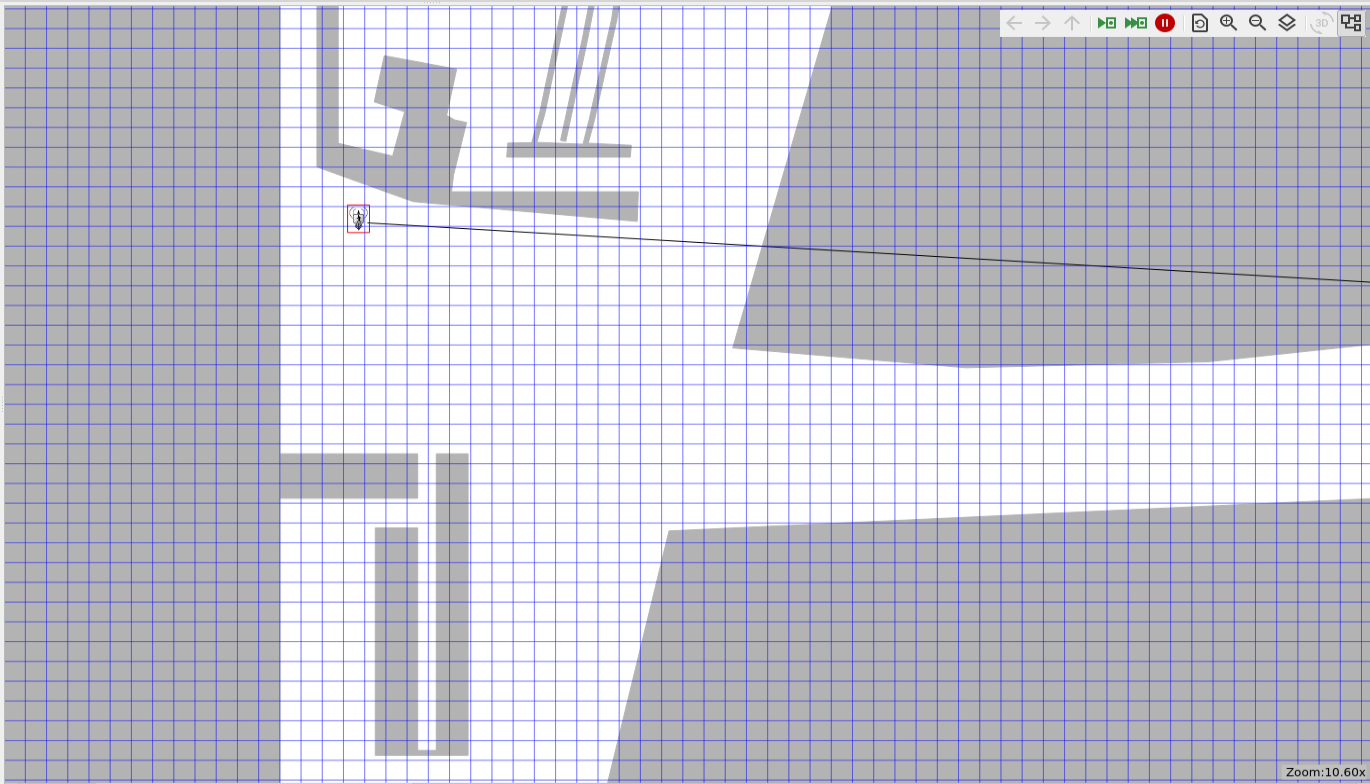
\includegraphics[width=3.2cm,clip,trim={9cm 0.4cm 23cm 12.5cm}]{./concept_2.png} };
\filldraw[fill=red!50!red!50,fill opacity=0.7, draw opacity=0.5] (7.45, 2.7) rectangle (7.8, 6.7);
\node[text width =5cm] at (7.6,8.5) {b) Cell-based density measurements};


\coordinate[] (station) at (8,-1);
\coordinate[] (p1) at (6.2,-5.3);
\coordinate[] (p2) at (9.2,-4.8);
\coordinate[] (p3) at (8.1,-3.2);
\coordinate[] (station2) at (7.9,-1);
\coordinate[] (p12) at (6.1,-5.3);
\coordinate[] (p22) at (9.3,-4.8);
\coordinate[] (p32) at (8.2,-3.2);



\draw[->]  (station) -- (p1) node[midway,left] {R};
\draw[->]  (station) -- (p2) node[midway, right] {R};
\draw[->]  (station) -- (p3) node[midway, left] {R};
\draw[->,purple]  (p2) -- (p1) node[pos=0.2,below] {D};
\draw[->,purple]  (p2) -- (p3) node[pos=0.5,left] {D};
\draw[->,purple]  (p3) -- (p1) node[pos=0.7,right] {D};

\draw[->, purple]  (station2) -- (p12) node[pos=0.65,left] {D};
\draw[->, purple]  (8.1,-1) -- (p22) node[pos=0.65, right] {D};
\draw[->, purple]  (8.1,-1) -- (p32) node[pos=0.65, left] {D};
\node[diamond,fill] at (station) {};
\draw[blue,fill=blue] (p1)   circle (2mm);
\draw[blue,fill=blue] (p2) circle (2mm);
\draw[blue,fill=blue] (p3)  circle (2mm);

\node[text width=5cm] (sa) at (8,0.1) {c ) Direct communication of density maps (D) and route recommendations (R)};

\node[text width=7cm] (sa) at (-0,8.5) {a) Layout: routes, measurement areas, relay node and base station};

\draw[-] (4.3,9) -- (4.3,-6);
\draw[-] (4.3,1.3) -- (10.3,1.3);
\end{tikzpicture}


\end{document}
